\chapter{Spectral Uplifting}

Although spectral rendering has multiple advantages, many renderers do not consider them to compensate for the ease of use and memory efficiency of the RGB representation. Even the physically-based phenomena can be ``faked'' by a few simple tricks, and therefore, many conventional rendering systems are RGB-based. This implies that most textures and materials created for renderers are RGB-based.

However, spectral renderers are still used both in the research and in the commercial sphere (e.g. ART, Mitsuba, Manuka). In comparison to an RGB-based texture, however, creating spectral textures is much more complicated and usually requires a real-life model whose reflectance spectra can be measured with a spectrometer, which is, in many cases, virtually impossible. 

The obvious solution is to convert the already existing RGB models to their spectral variants. We refer to this process as \emph{spectral uplifting}, however, other sources also use the term \emph{spectral upsampling}~\cite{sigmoidMethod}. 

By being able to uplift RGB values, we could utilize the RGB textures and materials and therefore eliminate the need for repeatedly creating the textures from scratch by the tedious process of measuring concrete spectral values.

However, converting an RGB value into its respective spectrum poses multiple difficulties. As the relationship between the spectral and RGB domain is not bijective (specifically, infinitely many spectral distributions render the same RGB values), distinctive approaches to the conversion process may render different spectral distributions. Although all of them might be correct in terms of the resulting RGB value, it is possible that none of them would be identical to spectral distribution measured with a spectrometer. This does not cause a problem under standard illuminant with regard to which the RGB values were uplifted. However, as already mentioned in , changing the illuminant causes distinct spectra to behave differently, which consequently results in \emph{metamerism}. Therefore, our uplifted spectra might behave differently than they would in real world. sem dam obrazok ak ho budem mat

We begin this chapter by reviewing the already existing approaches to spectral uplifting. We then talk about a new technique, \emph{constrained spectral uplifting}, which provides means for solving the above mentioned problems.

\section{Uplifting methods}

Although there have been multiple attempts at spectral uplifting, not many meet all the conditions required for a successful and complete conversion (e.g. one method may output reflectance spectra with values outside the (0,1) range, other method might work only for saturated colors etc.).

We base most of this section on an article by~\citet{upsamplingTechniques}, as it overviews multiple spectral uplifting techniques. It also proposes a new technique, which is considered to be the current state-of-the-art.

One of the first techniques was proposed by~\citet{upsamplingMacAdam}. The main goal of his research was to achieve the highest possible brightness for a given color saturation in printing. The uplifting process was only a byproduct of proof of limits to the brightness of colors, created especially for representing the reflectance of the researched colors (i.e colors of maximum brightness for any given saturation). Although this method is not limited to a specific input, it produces spectra that are box shaped and only consist of rising and falling edges. This type of representation is unsuitable for colors usually found in nature, which tend to have smooth spectra.

Another technique was proposed by~\citet{upsamplingSmits}. In this case, the uplifting is based on a box basis split into 10 discrete bins, which are derived using an optimization algorithm that accounts for energy conversion and aims for overall smoothness of the spectra. This approach is practically implemented and widely used, as it provides satisfactory results in the sRGB gamut in~\cite{upsamplingJakobHanika}. However, the uplifted spectra can acquire values above 1 in some cases, which does not satisfy the (0,1) range criterion. Furthermore, conversion of an RGB value to spectra and then back produces slight differences, which are amplified in scenes with multiple reflections. Lastly, this approach becomes unstable when used with wider gamuts, as it was not designed for this purpose.

The goal of the method by~\citet{upsamplingMeng} is wide-gamut uplifting. It also concentrates on optimizing the uplifting algorithm for spectral smoothness. However, it does not take energy conservation into account, which results in images with colors that have no physical counterpart (i.e. no real material could produce such colors). \citet{upsamplingMeng} tries to solve this by introducing a set of scaling methods for mapping the uplifted spectra to valid reflectances. These, however, fail if trying to uplift bright colors. 

One of the most recent uplifting techniques has been proposed by~\citet{upsamplingOtsu}. It is based on the observation that a typical measured reflectance spectrum can be represented with only a few principle components. The method uses clustered principal component analysis (PCA) and, unlike many other approaches, does not assume that spectra must necessarily be smooth. Such a simplification both eliminates the requirement of having a smoothness heuristic and enables the reconstructed spectra to match the actual measured spectra pretty well. This approach, however, also has its downsides. Firstly, the method does not satisfy the (0,1) range criterion, which, if clamped, results in color reproduction errors. Moreover, since there is no interpolation across clusters, similar RGB values might produce very different spectra, which might lead to discontinuities in rendering. However, in multiple cases, this method has been shown to outperform all of the already mentioned ones~\cite{upsamplingJakobHanika}.

A large part of this thesis is based on the work by~\citet{upsamplingJakobHanika}. We will therefore describe their approach in more detail.

In their article,~\citet{upsamplingJakobHanika} describe a parametric function space for efficient representation of spectral reflectance curves. They also show how to utilize such a space for the purposes of spectral uplifting.

The main goal was to create a spectral representation that would be both energy-conserving and would have a successful round-trip, i.e. the difference between the original RGB and the RGB obtained by conversion to spectra and back would be as small as possible. A simple analytical model has been created based on the equation specifying the DeltaE error created by round-trips. Spectra in accordance with this model are represented as following:
\begin{equation} \label{sigmoidRepresentation}
f(\lambda)=S(c_{0}\lambda^2+c_{1}\lambda+c_{2}),
\end{equation}
where $f(\lambda)$ is the resulting spectrum, $S$ is a simple sigmoid function and $c_{i}$ are coefficients of a second-order polynomial. Therefore, all spectra in this space are represented by three parameters.

In addition to energy conservation, the resulting spectra do not violate the (0,1) range constraint. They are extremely smooth and simple, which corresponds to many of the spectra typically found in nature. Another great advantage is memory efficiency, which requires only three values. However, representing spectra as specified in~\ref{sigmoidRepresentation} has its drawback. For example, there is currently no straightforward, well-defined computation of the RGB $\to$ spectrum conversion in such a domain. To uplift an RGB value, one must keep ``guessing'' the coefficients until the spectrum evaluates to the desired RGB.

In this specific implementation, the ``guessing'' process is performed mostly by the CERES solver~\cite{ceresSolver} (note:should I find out how this works?). It requires only an initial guess and a metric according to which it improves the guess (i.e. the DeltaE error originating from round-trips) and requires only a few iterations to converge to 0.

The uplifting process itself works by pre-computing RGB:spectra mappings and storing them in a texture. During rendering, only the required spectra are looked up in the texture.

In~\cref{alg:upliftingAlgSigmoid}, we describe the pseudo-algorithm of the uplifting process, which is very similar to the one used in our implementation.
\begin{algorithm}[t]
	\caption{Spectral uplifting by~\citet{upsamplingJakobHanika}}
	\label{alg:upliftingAlgSigmoid}
	\begin{algorithmic}[1]
		\State create $RGBCube$ with empty RGB:spectra mappings
		\State $unfittedPoints \gets$ a list of all points in $RGBCube$
		\State $centerPoint \gets$ index of the middle of $RGBCube$
		\Statex \Comment{$RGBCube[centerPoint].rgb \simeq (0.5,0.5,0.5)$}
		\State $centerPoint.coefficients \gets (0,0,0)$
		\Statex \Comment ``guess'' the coefficients at $centerPoint$
		\State run the CERES optimizer for $RGBCube[centerPoint]$
		\State remove $RGBCube[centerPoint]$ from $unfittedPoints$
		\While {$unfittedPoints$ is not empty}
		\ForAll{$point \in unfittedPoints$}
		\If{$point$ has a neighbor $v$ with defined coefficients}
		\State $point.coefficients \gets v.coefficients$
		\State run the CERES optimizer for $point$
		\If{optimization was successfull}
		\State remove $point$ from $unfittedPoints$
		\EndIf
		\EndIf
		\EndFor
		\EndWhile
	\end{algorithmic}
\end{algorithm}

This means that the cube is optimized from the middle.

Obviously, not all rgb values can be uplifted as such. However, jakob says that we need only 64 dimensions and that, as the sigmoid curves are very similar, the middle values can be interpolated (show algorithm). 

Another drawback is the limitation of such a spectral representation to only smooth spectra with no sharp edges. We discuss this specific issue in detail in ref, where we provide arguments as to why we do not use the sigmoid representation later in our thesis.

This technique, in comparison to other existing techniques, has definitely the best error (maybe show image).
the results are obviously metameric, show pictures

alisa bases her approach on this thing

\begin{figure}[t!]
	\centering
	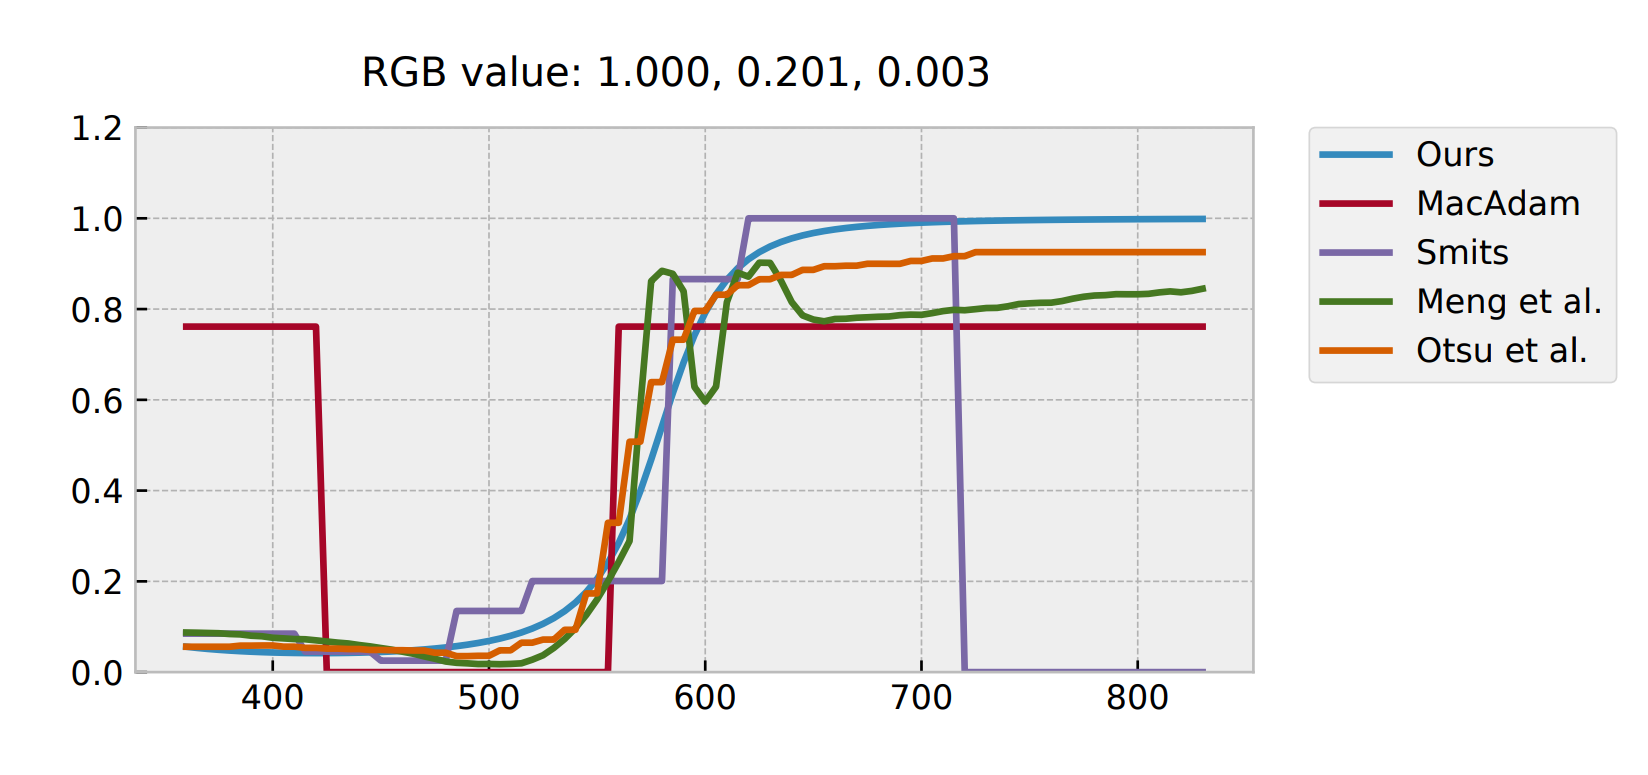
\includegraphics[width=0.8\linewidth]{img/upsampling_techniques.png}
	\caption{Comparison of spectral uplifting techniques as shown by~\citet{upsamplingJakobHanika}. All spectra were created by uplifting the (1, 0.201, 0.003) RGB value and the results were plotted according to the corresponding techniques. The ``Ours'' approach, in this case, refers to the approach by~\cite{upsamplingJakobHanika}.}
	\label{fig:upliftingTechniques}
\end{figure}

\section{Constrained spectral uplifting}

Achieving identity of our uplifted spectra to the real-world spectra is, obviously, impossible. However, uplifting many RGB-based models does not require us to be able to uplift the whole RGB gamut, but only the color spectrum used for the creation of said models. As it is pretty common for the artists in the VFX modeling industry to use specific color atlases when designing textures and materials, the ability to \emph{constrain} the uplifting system with these base colors would be extremely useful in such cases.

In other words, the user would define specific RGB:spectra mappings which would later be used in order to uplift certain RGB triplets. RGB values that would not have a pre-defined mapping would be uplifted by altering the curves of their neighbors that already have a mapping. 

We call this process \emph{constrained spectral uplifting}. Although it does not provide as much freedom as other spectral uplifting approaches, it works for our benefit in terms that the results would not be a subject to high metamerism, which is, after all, the goal of this thesis.

Following, we provide a brief overview of the algorithm used for constrained spectral uplifting:
\begin{enumerate}[label=S.\arabic*]
	\item \emph{RGB cube initialization} --- create an RGB cube that will be used as a structure for storing the RGB:spectra mappings. For every RGB triplet in the cube, initialize its respective spectrum to empty.
	\item \emph{seeding the cube} --- store the input spectra at the lattice points with their respective RGB values.
	\item \emph{sampling of the spectra} --- for each spectrum, sample it so it can be represented (and also reconstructed) with a small, constant number of parameters. Save the parameters instead of the spectrum.
	\item \label{Step 4} \emph{spectra approximation at other lattice points} --- use the already existing parameters in the cube to reconstruct RGB values at lattice points that do not have a defined spectrum yet. For this purpose, an approximation algorithm must be used.
\end{enumerate}
In addition to memory efficiency, sampling spectra is essential for the approximation process mentioned in~\ref{Step 4}. We explain the reasoning behind this in ref3. For now, we assume that the spectra must be stored as efficiently as possible, with constant number of parameters.

we base our process on jakob and hanika, but we constrain the input and we also choose a different sampling method.

\subsection{Spectral sampling}

In real world, the spectral reflectance curve is a continuous function obtaining values in range (0,1). As it does not have to be necessarily smooth storing any kind of function in any kind of digital system requires its discretization.


Also, probably here is a good time to mention that we are focusing on the reflectance spectra, however we will also talk about emission spectra in this section solely for research purposes

In many spectral renderers,  

\subsubsection{Available methods}

\subsubsection{Trigonometric moment method}

A review of the moment method (basically just a review of the paper)

